\begin{appendices}
\chapter{Типы картин мира} \label{AppendixA}

В соответствие с предыдущим параграфом в результате работы механизмов самоорганизации на множестве знаков формируются три основных типа структур. Каждую из них в соответствии с \cite{Osipov1990} будем называть неоднородной семантической сетью или, поскольку это не приводит к недоразумениям, семантической сетью. Рассмотрим три таких сети.
\begin{enumerate}
	\renewcommand\labelenumi{\theenumi.}
	\item Семантическую сеть $H_P=\langle 2^P,\mathfrak R_P\rangle$ на множестве образов, где $\mathfrak R_P=\{R_1,R_2,R_3,R_4\}$ "--- семейство отношений на образах.
	\item Семантическую сеть $H_A=\langle 2^A,\mathfrak R_A\rangle$ на множестве личностных смыслов, где $\mathfrak A=\{R_5\}$ "--- семейство отношений на личностных смыслах.
	\item Семантическую сеть $H_M=\langle 2^M,\mathfrak R_M\rangle$ на множестве значений знаков, где $\mathfrak R_M=\{R_1^\prime,R_3^\prime,R_6,R_7\}$ "--- семейство отношений на значениях.
\end{enumerate}

Тройку объектов $H=\langle H_P,H_A,H_M\rangle$ будем называть семиотической сетью. Переходы между сетями $H_P$, $H_A$, $H_M$ реализуются, как следует из предыдущего, посредством процедур $\Psi_m^a$, $\Psi_a^p$ и $\Psi_p^m$.

Уровень имён знаков может наследовать каждую из описанных выше семантических сетей. Благодаря такому наследованию можно говорить о формировании той или иной семантической сети на уровне знаков (не только на уровне их компонент).

Предлагается выделять три типа картины мира: рациональную, житейскую и мифологическую \cite{Chudova2012}. 
Мы видели, что на сети $H_P$ можно определить операции обобщения (и классификации) по признакам (раздел \ref{subsect_2_3_1}). Именно эти операции характерны для рациональной картины мира. На основании этих соображений и ряда психологических экспериментов (описание которых остаётся за пределами настоящего доклада) можно полагать, что именно сеть на множестве образов (и ее наследование на уровень имён знаков) лежит в основе рациональной картины мира. Здесь надо подчеркнуть важность слов <<в основе>>. Все типы картин мира используют сети на образах, на смыслах и сценариях, но есть некоторая <<управляющая>> сеть, которая служит для формулирования цели, поиска подходящих действий, вызова сценариев и изменения личностных смыслов. Например, в рациональной картине мира в сети на образах выполняется выработка цели, затем в сети на значениях находятся подходящие роли в сценарии как условия выполнения действий для достижения цели, далее учитываются смыслы объектов, которые могут быть мотивами или препятствиями, или средствами для достижения цели \cite{Chudova2014}. Отметим, что могут быть описаны и вырожденные картины мира, в которых используются не три, а только две сети (например, только $H_A$ и $H_M$ для нигилистической картины мира \cite{Chudova2012}). 

Житейская картина мира характеризуется следованием некоторым стереотипам или сценариям поведения. Таким образом, наследование на уровень имён знаков сети на значениях приводит к формированию житейской картины мира. Здесь также следует отметить, что сеть на значениях является лишь ведущей: моделирование, например, картины мира чиновников реализуется на двух сетях "--- сценариев и личностных смыслов. Поэтому при возникновении нового предмета потребности (например, выделение бюджета на науку и культуру) находится сценарий, в котором смысл цели из амбивалентного превращается в смысл препятствия. Поскольку в этом процессе не присутствуют образы, то речь идёт о вырожденной картине мира. В общем случае в житейской картине мира выбранный сценарий (на сети значений) пополняется образами тех объектов (в том числе партнёров), которые наилучшим образом (в соответствии с оценкой на сети смыслов) могут исполнять записанные в сценарии роли (например, начальник подбирает исполнителей в новую группу для <<хорошего>> выполнения нового вида работ или жених и невеста составляют список гостей на свадьбу в соответствии со своими представлениями о том, как должна выглядеть <<хорошая>> свадьба).

В мифологической картине мира каждая роль имеет неизменный смысл и заданный образ, т.е. ведущей в этом случае является сеть на смыслах. Иначе говоря, наследование сети $H_A$ на уровень имён знаков приводит к формированию мифологической картины мира.

\chapter{Модель функции целеполагания на синтаксическом уровне} \label{AppendixB}

Задача управления поведением субъекта деятельности включает в себя фазы планирования и исполнения плана \cite{Osipov2002c,Osipov2003a,Osipov2008b}. Первая задача планирования заключается в выдвижении цели "--- целеполагании. Применим развитый выше аппарат к решению этой задачи. Синтез плана и его исполнение будут рассмотрены во второй части статьи.
Целеполагание "--- сложный процесс, который включает в себя не только выдвижение цели, но и определение условий и конкретного способа ее достижения. Как уже было сказано, характер процесса целеполагания определяется типом картины мира (КМ) субъекта. В случае житейской КМ ведущим компонентом является значение, т.е. субъект отталкивается от сюжетно"--~ролевой структуры и использует уже существующие знаки, чтобы выбрать подходящую ситуацию, которая и будет целевой.
Для обозначения операции переходов на сети значений, образов и личностных смыслов введём недетерминированный оператор переходов $Tr$, действующий на булеанах $2^P$, $2^A$ и $2^M$: $Tr(x)=x^\prime$, где $x,x^\prime\in 2^A$ или $x,x\prime\in 2^P$, или $x,x^\prime\in 2^M$. Левая композиция оператора $\Psi_x^y$, где $x\in\{m, a, p\}$, $y\in\{m, a, p\}$ (т.е. любого из операторов  $\Psi_p^m$, $\Psi_m^a$ или $\Psi_a^p$), с оператором переходов по сети $y$ обозначим как $\underline{\Psi}_x^y:\underline{\Psi}_x^y=\Psi_x^y\circ Tr(x)$, где $Tr(x)=x^\prime$, $x\in 2^A$ или $x\in 2^P$, или $x\in 2^M$ и $x^\prime\in 2^A$, или $x^\prime\in 2^P$, или $x^\prime\in 2^M$. Под композицией операторов будем понимать применение левого оператора к результату применения правого оператора. Правая композиция оператора $\Psi_x^y$ , где $x\in\{m, a, p\}$, $y\in\{m, a, p\}$, с оператором переходов по сети y обозначим как $\overline{\Psi}_x^y: \overline{\Psi}_x^y=Tr(y)\circ\Psi_x^y$, где $Tr(y)=y^\prime$, $y\in 2^A$ или $y\in 2^P$, или $y\in 2^M$ и  $y^\prime\in 2^A$, или $y^\prime\in 2^P$, или $y^\prime\in 2^M$. Например, левая композиция оператора   с оператором перехода по сети образов запишется как $\underline{\Psi}_p^m=\Psi_p^m\circ Tr(y)$.

Процесс целеполагания осуществляется в рамках какой-либо деятельности. Будем рассматривать случай, когда мотив деятельности осознан, т.е. знак предмета потребности включён в картину мира субъекта деятельности. Тогда мотивом деятельности (в житейской картине мира) является значение ($m$) этого знака. Мотив удовлетворяется, когда существует знак, такой, что результатом применения правой композиции оператора   с оператором переходов ($Tr(p)\circ\Psi_a^p$) к личностному смыслу этого знака является образ знака предмета потребности. (Или на семантическом уровне: существует знак, такой, что результатом некоторого действия, интерпретирующего личностный смысл этого знака, выступает образ знака предмета потребности.)

Тогда знак, результатом применения к которому правой композиции оператора $\Psi_a^p$ с оператором переходов является образ знака предмета потребности, будем называть целевым знаком. Или на семантическом уровне: целевым будем называть такой знак, в структуре личностного смысла которого существует действие, применение которого приводит к формированию признаков образа предмета потребности (удовлетворению потребности). Процесс целеполагания, таким образом, заключается в построении такой последовательности знаков, которая заканчивается знаком, из которого достижим мотив, т.е. удовлетворяется потребность.

В соответствии с разд. 3.4 значение знака будем представлять в виде множества пар <<действие "--- роль предмета в этом действии>>, образ ($p$) такого знака "--- в виде набора свойств, т.~е. пар <<признак "--- значение признака>>, личностный смысл ($a$) "--- в виде правила, соответствующего действию субъекта с предметом; условие и эффект действия такого правила задаются в виде множества свойств.

Далее, $s^*$ "--- знак, экземпляр значения которого $\mu^*$ является мотивом деятельности. В приведённом ниже алгоритме целеполагания будем использовать как синтаксические, так и семантические соображения, особенно не подчёркивая этого обстоятельства.

\textbf{Алгоритм GS.}

\textbf{Вход}: знак предмета потребности $s^*$, мотив $\mu^*$.

\textbf{Шаг 1}: переход $\mu^*\rightarrow a_1$ (применяется оператор $\underline{\Psi}_m^a$). На подсети значений (в сценарии с порождающим знаком $s^*$) применяем к $\mu^*$ оператор переходов $Tr$ до тех пор, пока не будет получено такое значение $m_1$, знак $s_1$ которого обладает личностным смыслом $a_1$ таким, что интерпретирующее его действие в множестве добавляемых признаков $p_{add}$ содержит множество признаков $p^*$ знака $s^*$:  $\underline{\Psi}_m^a:\mu^*\rightarrow a_1$, где $a_1$ такое, что $p^*\subseteq p_{add}(a_1)$ (применение операторов $Tr(\mu^*)$ и $\Psi_m^a$ на рис. \ref{fg:goalsetting_alg}). Если знак $s_1$ не совпадает со знаком $s^*$, то найденный целевой знак со своим личностным смыслом является целью и алгоритм завершает работу, иначе переходим к шагу 2.

\textbf{Шаг 2}: переход $a_1\rightarrow\bar p_2$  (применяется оператор $\overline{\Psi}_a^p$). На подсети образов применяем оператор переходов $Tr$ к образу, содержащему один или несколько признаков условия $p_{cond}$ правила, интерпретирующего личностный смысл $a_1$ знака $s_1$ до тех пор, пока не будет получено максимального по мощности множества признаков $p_2$ знака $s_2$, являющегося подмножеством $p_{cond}$. Объединение признаков образа $p_2$ знака $s_2$ с каким-либо признаком (одним или несколькими) из множества $p_{cond}\\p_2$ будем называть расширенным образом $\bar p_2$: $\overline{\Psi}_a^p:a_1\rightarrow\bar p_2$, где $\bar p_2$ такое, что $p_2\subseteq\bar p_2$  и  $\bar p_2\subseteq p_{cond}$ (применение операторов $\Psi_a^p$ и $Tr(p_1)$ на рис. \ref{fg:goalsetting_alg}).

\textbf{Шаг 3}: переход $\bar p_2\rightarrow\mu_3$ (применяется оператор $\overline{\Psi}_p^m$). На подсети значений применяем оператор $Tr$ к какому-либо значению знака $s_3$, образ которого совпадает с множеством признаков $\bar p_2\\p_2$ до тех пор, пока не будет получено такого экземпляра $\mu_3$, что:
\begin{itemize}
	\item порождаемый знаком $s_3$ (с первым по порядку $\geqslant$ экземпляром значения $\mu_3$ в $M_{scen}$) элементарный сценарий $M_{est}(s_3)$ совпадает с каким-либо элементарным сценарием (с первым по порядку $\geqslant$ экземпляром значения $\mu^\prime_2$ в $M_{scen}$), порождаемым знаком $s_2$, найденным на шаге 2 с точностью до знаков $s_2$ и $s_3$ (т.е. без их учёта);
	\item соответствующий экземпляру значения $\mu_3$ личностный смысл $a_3$ интерпретируется таким действием, что в множество признаков его эффекта включено множество признаков образа $p_3$ самого знака $s_3$: $\overline{\Psi}_p^m:\bar p_2\rightarrow\mu_3$, где $\mu_3$ "--- первый по порядку экземпляр значения в множестве $M_{scen}$ сценария $M_{est}(s_3)$, причём   такой, что $M_{est}(s_2)=M_{est}(s_3)$ без учёта знаков $s_2$ и $s_3$ (применение операторов $Tr(p_2)$, $\Psi_p^m$ и $Tr(\mu_3)$ на рис. \ref{fg:goalsetting_alg}).
\end{itemize}

\textbf{Шаг 4}: переход $\mu^\prime_2\rightarrow a_2$ (применяется оператор $\Psi_m^a$). Нахождение личностного смысла $a_2$, соответствующего значению $\mu^\prime_2$ знака $s_2$. Завершение работы алгоритма.

\textbf{Выход}: либо знак $s_1$ и его личностный смысл $a_1$, либо знак $s_2$ и его личностный смысл $a_2$.

В результате работы алгоритма найден знак $s_2$, не совпадающий со знаком предмета потребности $s^*$, личностный смысл $a_2$ которого интерпретируется действием, приводящим к удовлетворению потребности. Целью, таким образом, становится знак $s_2$ с личностным смыслом $a_2$ (рис. \ref{fg:goalsetting_alg}).

\begin{figure}[h]
	\centering
	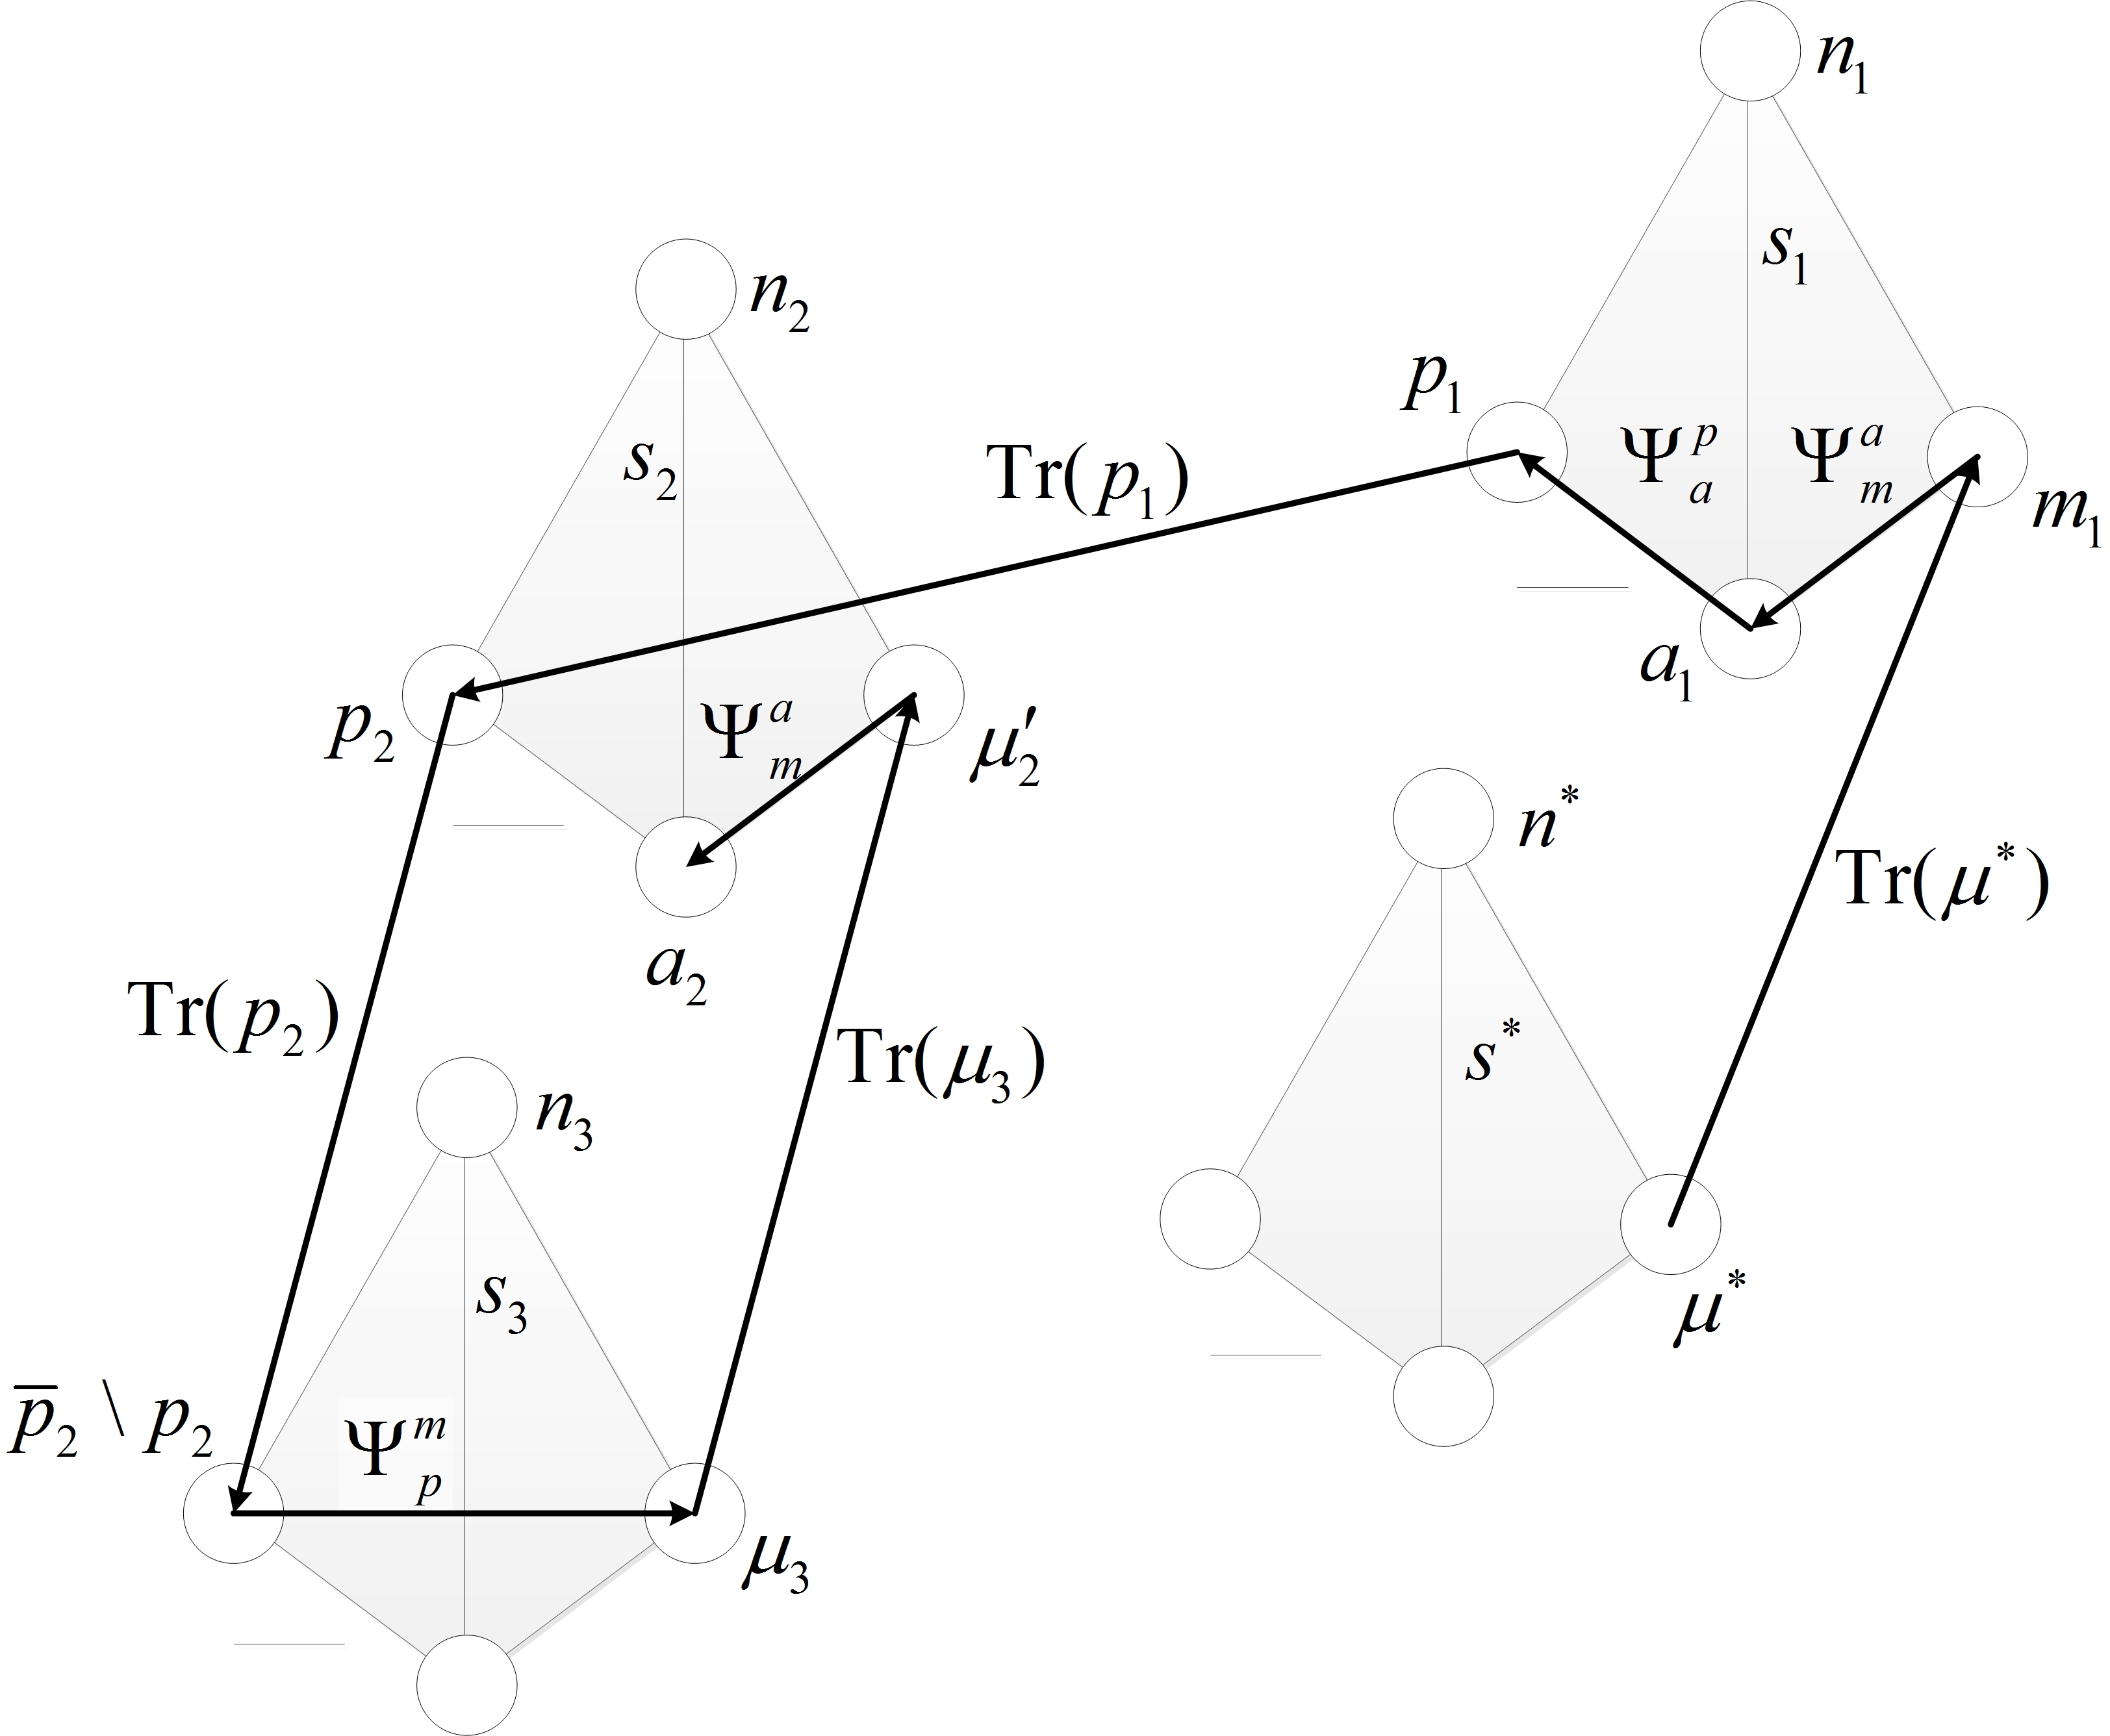
\includegraphics[width=\linewidth]{goalsetting_alg.jpg}
	\caption[]{Иллюстрация к алгоритму целеполагания: $s^*$ "--- знак предмета потребности, $\mu^*$ "--- экземпляр его значения, иначе говоря, мотив деятельности. Стрелками обозначены операторы $\Psi_p^m$, $\Psi_m^a$, $\Psi_a^p$ и $Tr$.}
	\label{fg:goalsetting_alg}
\end{figure}

\textbf{Пример}. Опишем в качестве простого примера процедуру целеполагания руководителя команды разработчиков программного обеспечения (рис. \ref{fg:goalsetting_ex}).

\begin{figure}[h]
	\centering
	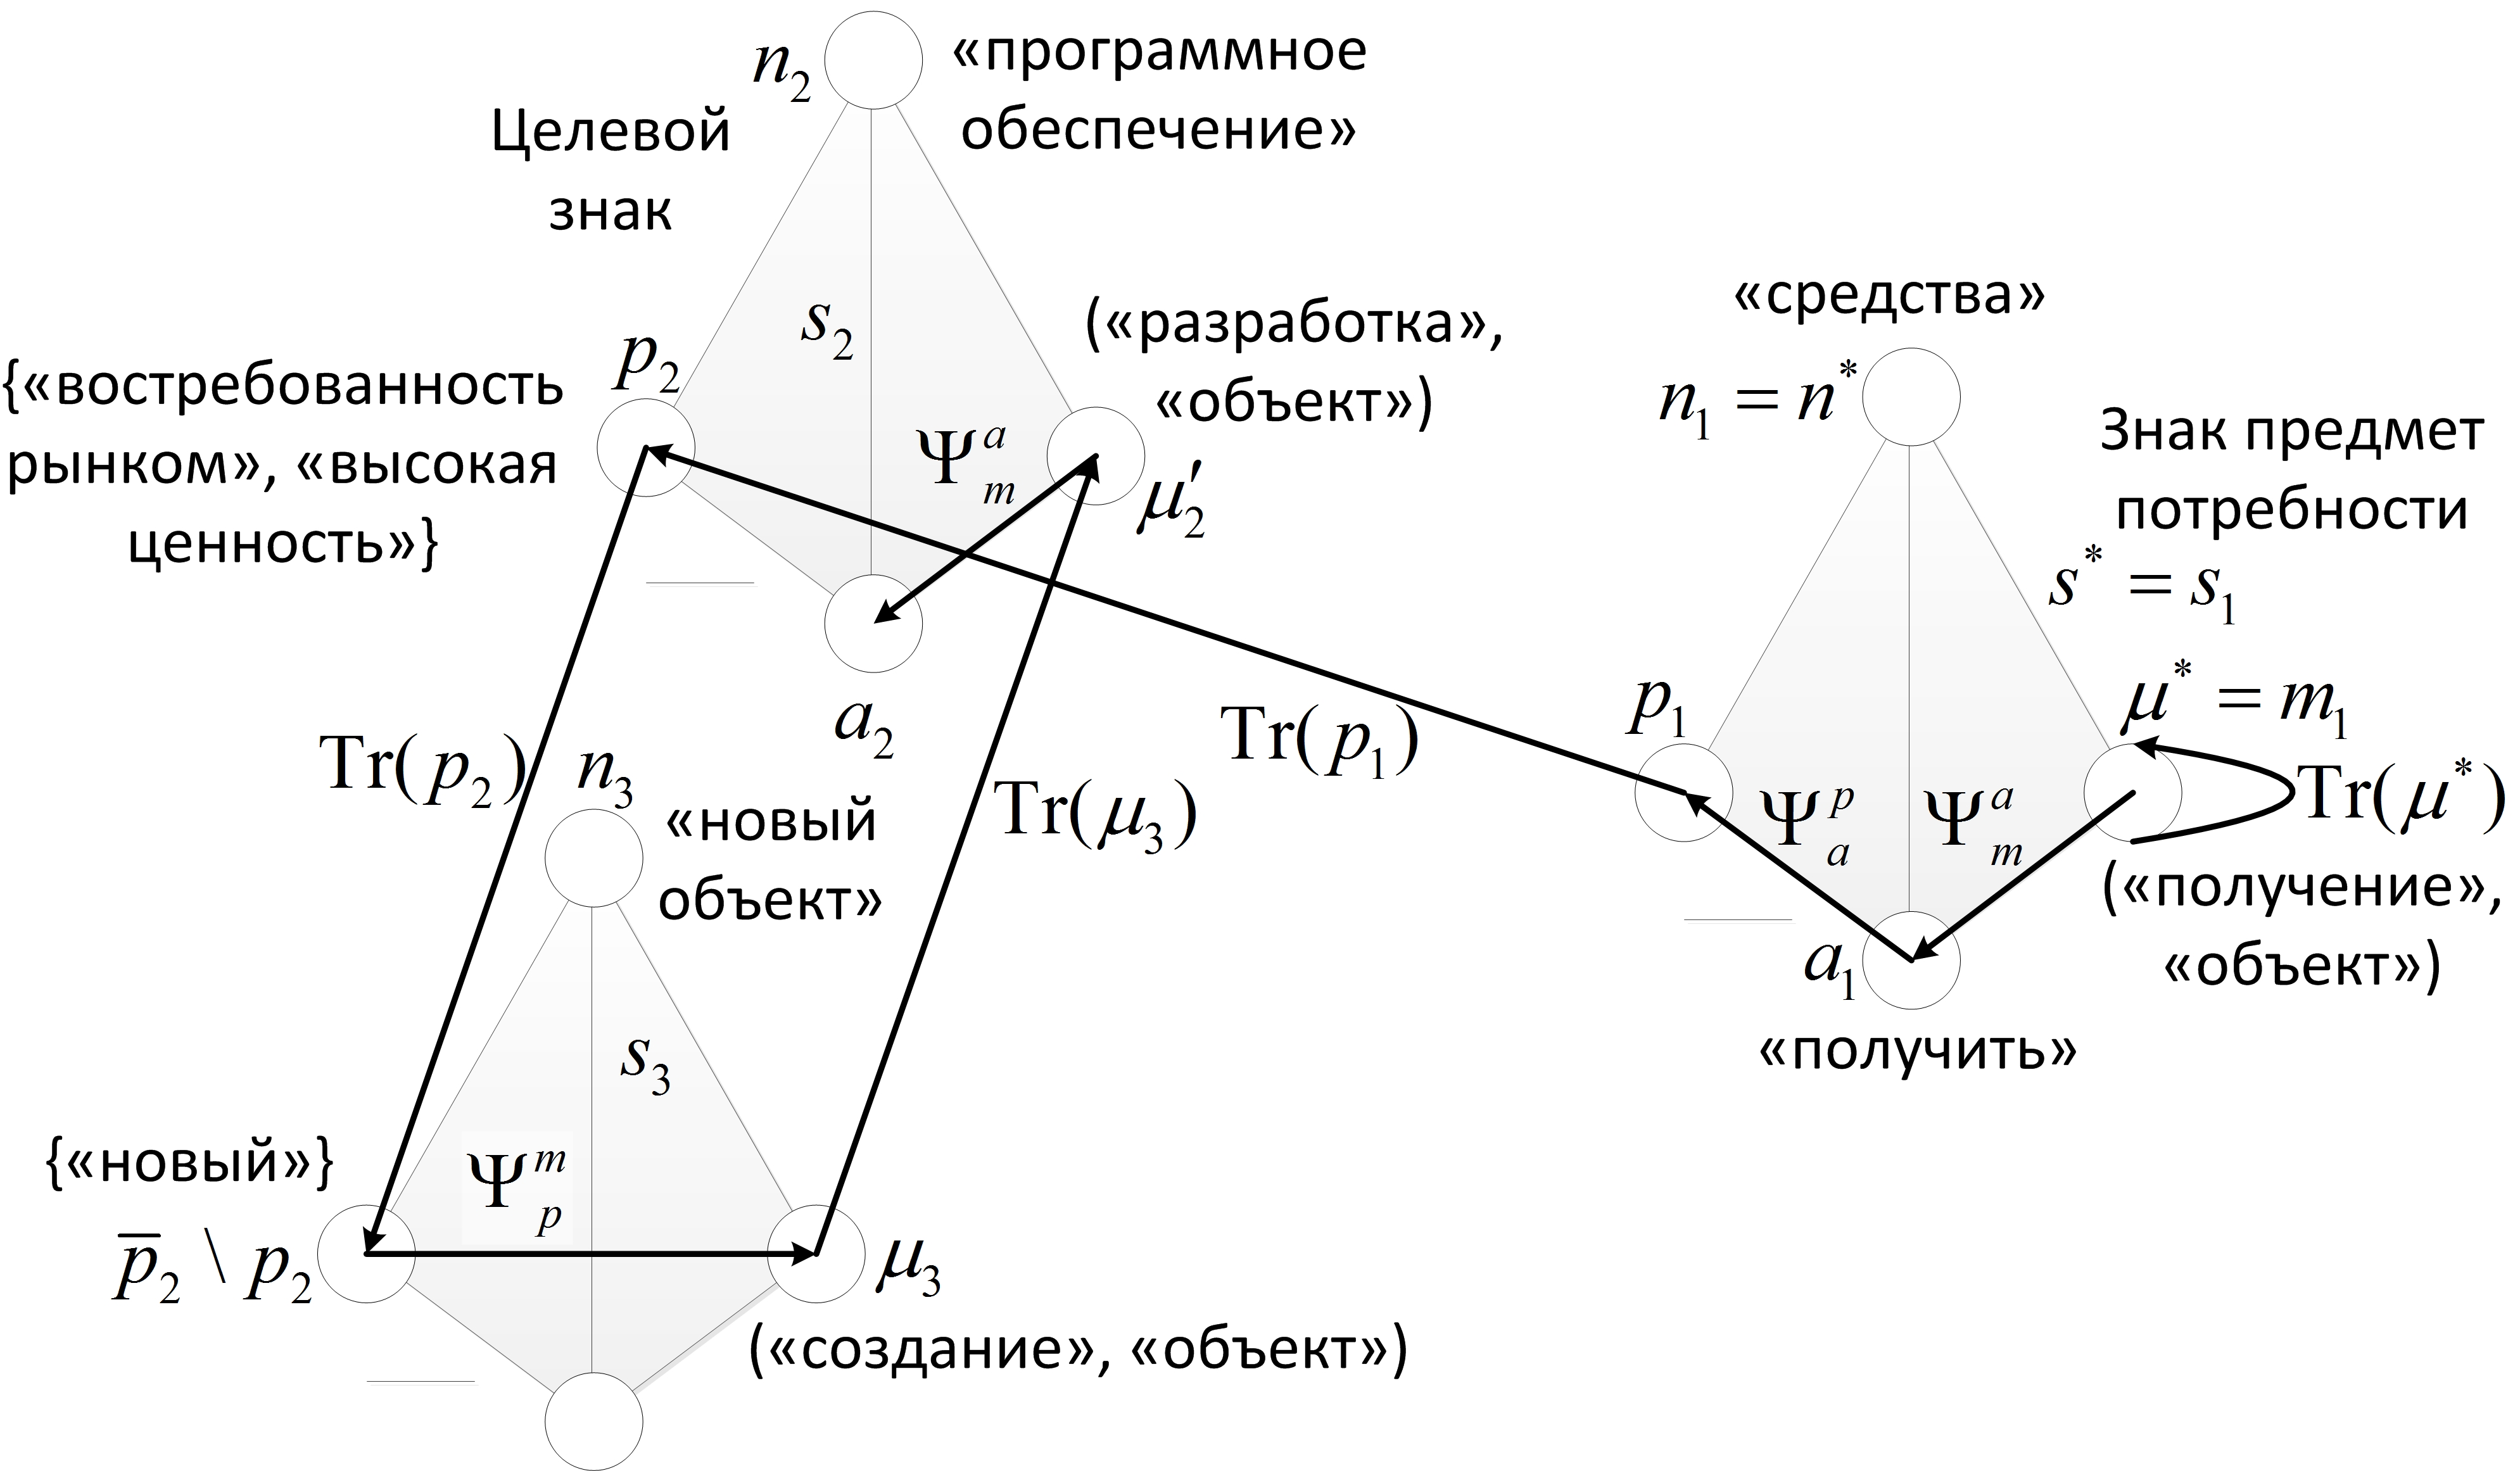
\includegraphics[width=\linewidth]{goalsetting_ex.jpg}
	\caption[]{Пример процесса целеполагания руководителя команды разработчиков с житейской картиной мира. Знаком предмета потребности руководителя является знак с именем <<средства>>. Стрелками обозначены операторы $\Psi_p^m$, $\Psi_m^a$, $\Psi_a^p$ и $Tr$.}
	\label{fg:goalsetting_ex}
\end{figure}

Руководитель команды использует в данном случае житейскую картину мира, мотивом его деятельности является значение знака <<средства>>, один из экземпляров значения которого "--- <<получение>>, обладающее семантической валентностью <<объект>>. Иначе говоря, один из экземпляров значений знака средства есть пара (<<получение>>, <<объект>>). Предположим, образ этого знака содержит признаки: <<высокая ценность>>, <<востребованность рынком>>, <<новое>>.

\textbf{Алгоритм GS.}

\textbf{Вход}: знак <<средства>> и мотив (<<получение>>, <<объект>>).

\textbf{Шаг 1}: переход значение "--- личностный смысл. Сценарий образуется семантическими валентностями предикатного слова, (в данном случае "--- <<получение>>). Субъект ищет знак, при этом его личностный смысл интерпретируется действиями, которые он будет осуществлять, чтобы удовлетворить мотив. Иначе говоря, в множестве добавлений правила, интерпретирующего личностный смысл, должны содержаться необходимые признаки предмета, за который происходит получение средств, например <<высокая ценность>>, <<востребованность рынком>>, <<новое>> и т.д. Предположим, что будет найден личностный смысл <<получить>> знака <<средства>>.

\textbf{Шаг 2}: переход личностный смысл "--- образ. Выполнение действия, соответствующего найденному личностному смыслу, требует удовлетворения признаков из условия действия. Происходит поиск такого знака, образ которого содержит необходимые признаки. Так как руководитель команды разработчиков имеет дело с программным обеспечением, то рано или поздно им будет найден знак <<программное обеспечение>>, так как его образ содержит признаки <<высокая ценность>>, <<востребованность рынком>>. Неудовлетворённые признаки из условия правила вместе с удовлетворёнными образуют расширенный образ, например <<новое программное обеспечение>>.

\textbf{Шаг 3}: переход образ "--- значение. Ищется знак, содержащий в образе признак <<новый>>, например знак <<новый объект>>. Выбираем экземпляр значения этого знака. Экземпляр значения должен быть первым в каком-либо сценарии, совпадающим с каким-либо сценарием знака <<программное обеспечение>>. Таким экземпляром может служить <<создание>>, так как в картине мира руководителя команды имеется необходимый сценарий. Для соответствующего сценария, порождённого знаком <<программное обеспечение>>, первым экземпляром в таком случае выступает <<разработать>>.

\textbf{Шаг 4}: переход значение "--- личностный смысл. Выбирается личностный смысл знака <<программное обеспечение>>, соответствующий экземпляру значения <<разработать>>. Действие, интерпретирующее этот личностный смысл, в множестве добавляемых признаков будет включать признаки <<высокая ценность>>, <<востребованность рынком>>, <<новое>>, содержащиеся в образе знака <<средства>> и удовлетворяющие мотив. Таким образом, текущий знак является целевым, а целью "--- пара <<разработать>> "--- <<программное обеспечение>>.

\textbf{Выход}: знак <<программное обеспечение>> и его личностный смысл <<разработать>>.
\end{appendices}